\section{Accessibility to healthcare services}

\subsection{Italian overview}

\begin{frame}
	\frametitle{Accessibility to healthcare services in Italy}
	
	\begin{figure}[h]
		\centering
		\subfloat[Acc. to the closest centre]{
			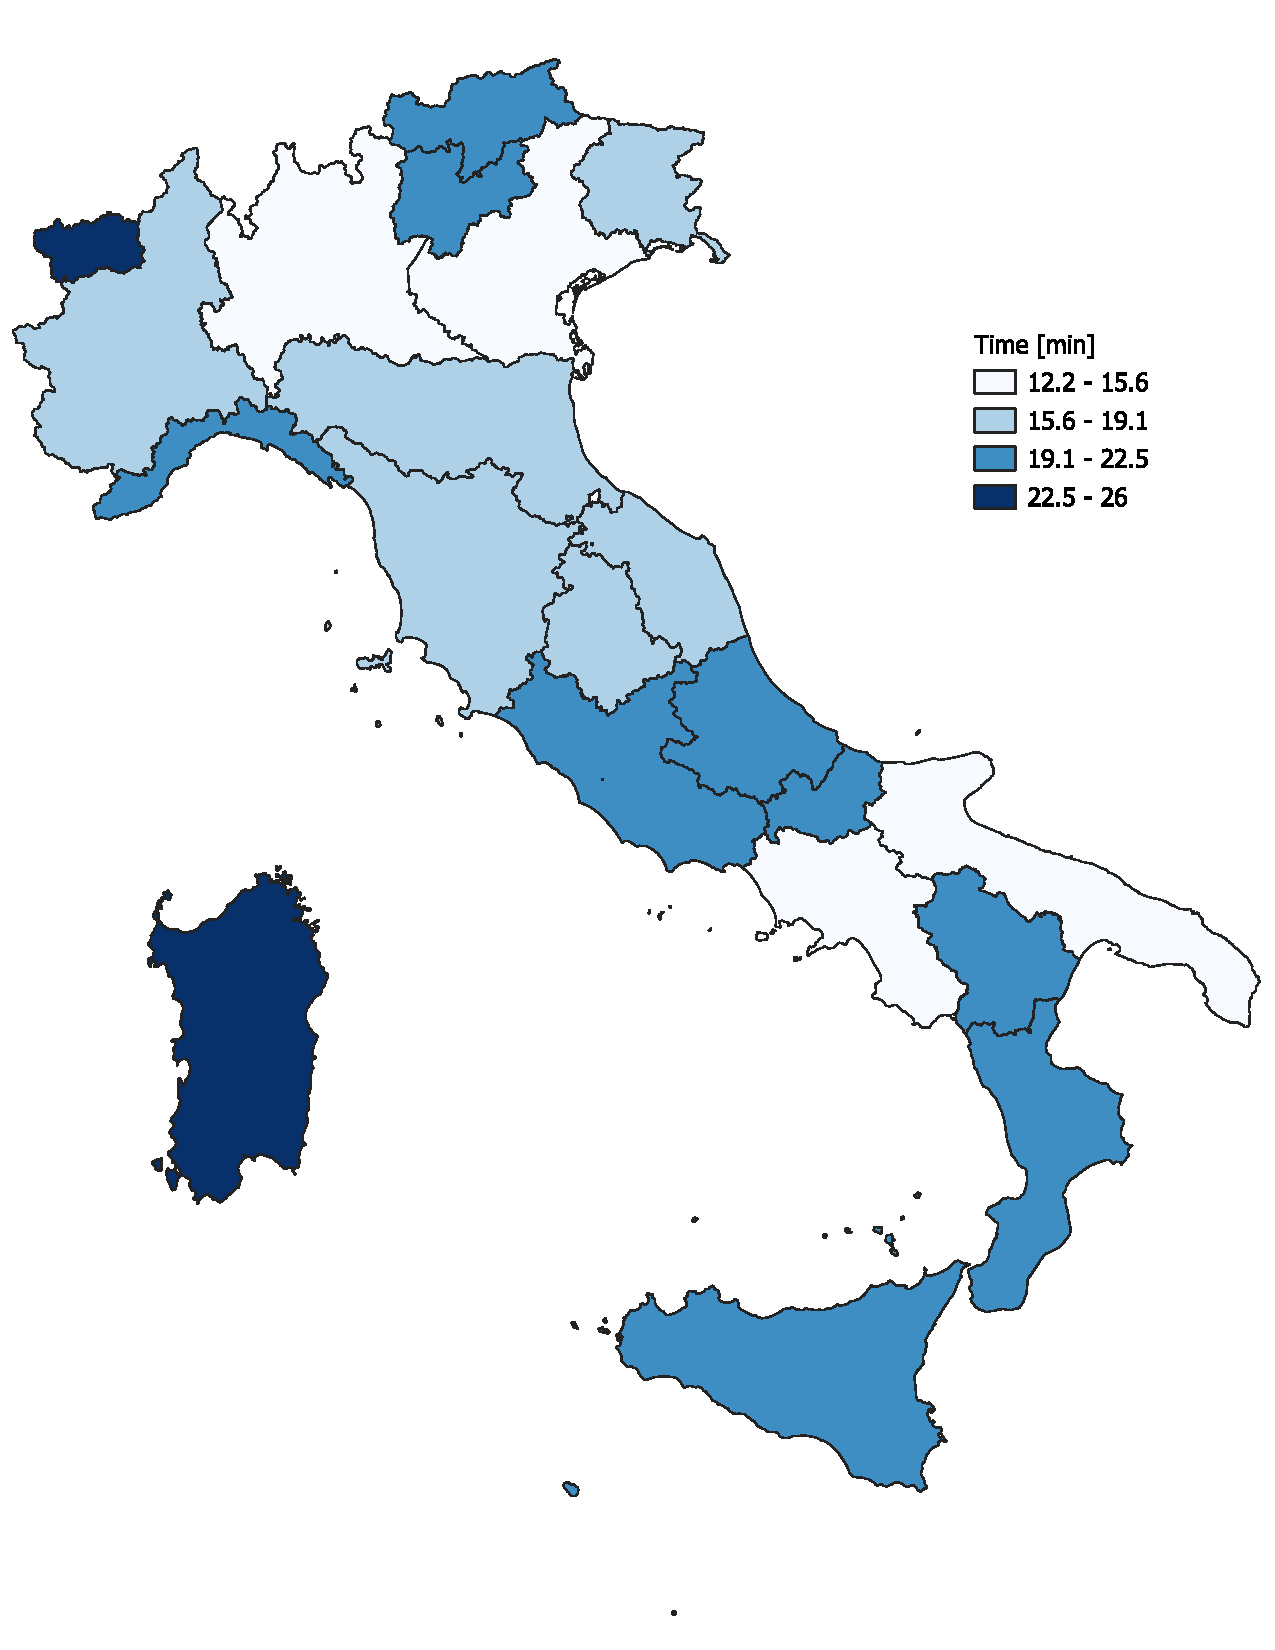
\includegraphics[width=0.4\textwidth]{../report/img/Accessibilità per regione.pdf}
		}
		\subfloat[Acc. to the 3 closest centres]{
			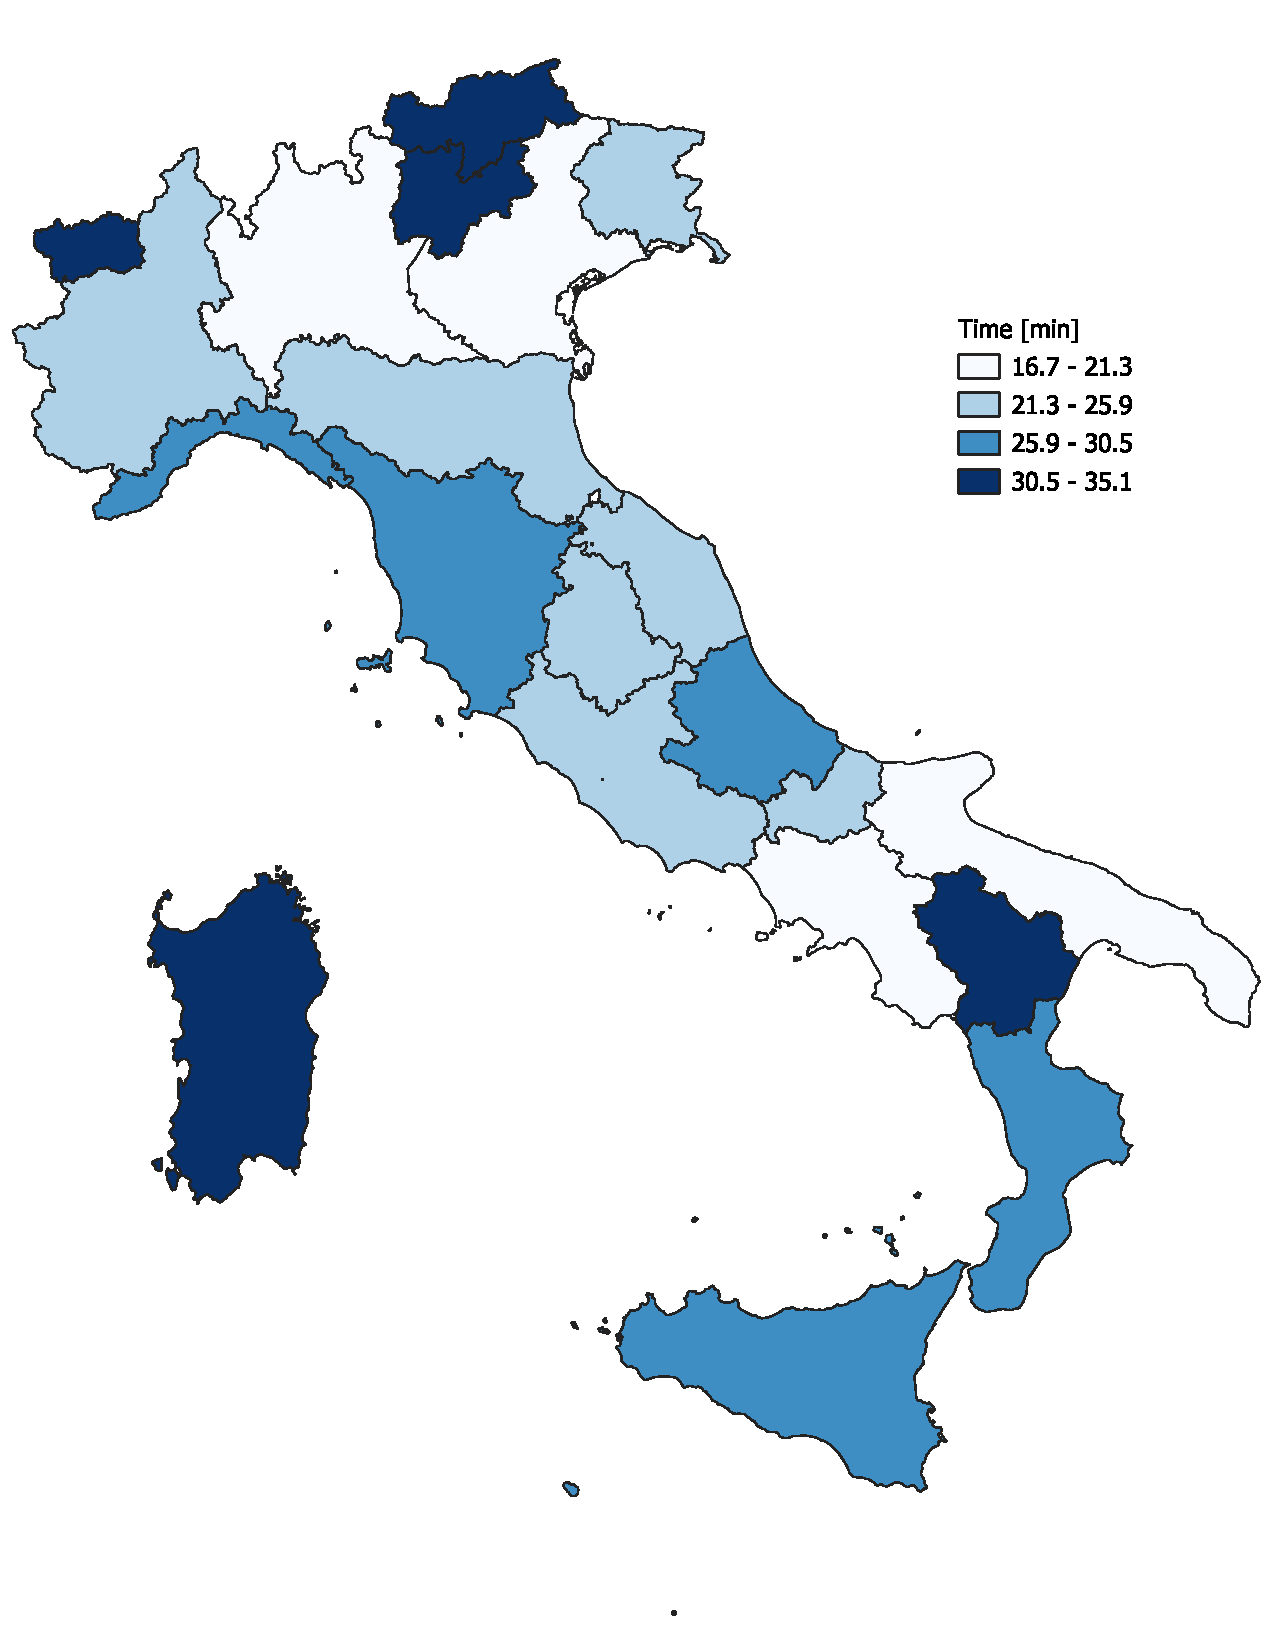
\includegraphics[width=0.4\textwidth]{../report/img/Accessibilità per regione n3.pdf}
		}
	\end{figure}
	
\end{frame}


\subsection{North of Italy}

\begin{frame}
	\frametitle{Categories based on travel time}
	
	Access time divided in 4 categories:
	
	\begin{center}
		\begin{tabular}{l c l}
			\toprule
			\textbf{No.} & \textbf{Travel time} & \textbf{Accessibility}\\
			& [min] & \\
			\midrule
			1 & < 15 & High\\
			2 & [15, 30) & Medium-high\\
			3 & [30, 45) & Medium-low\\
			4 & > 45 & Low\\
			\bottomrule
		\end{tabular}
	\end{center}
	
\end{frame}


\begin{frame}
	\frametitle{Accessibility in the North of Italy (1)}
	
	\begin{figure}[h]
		\centering
		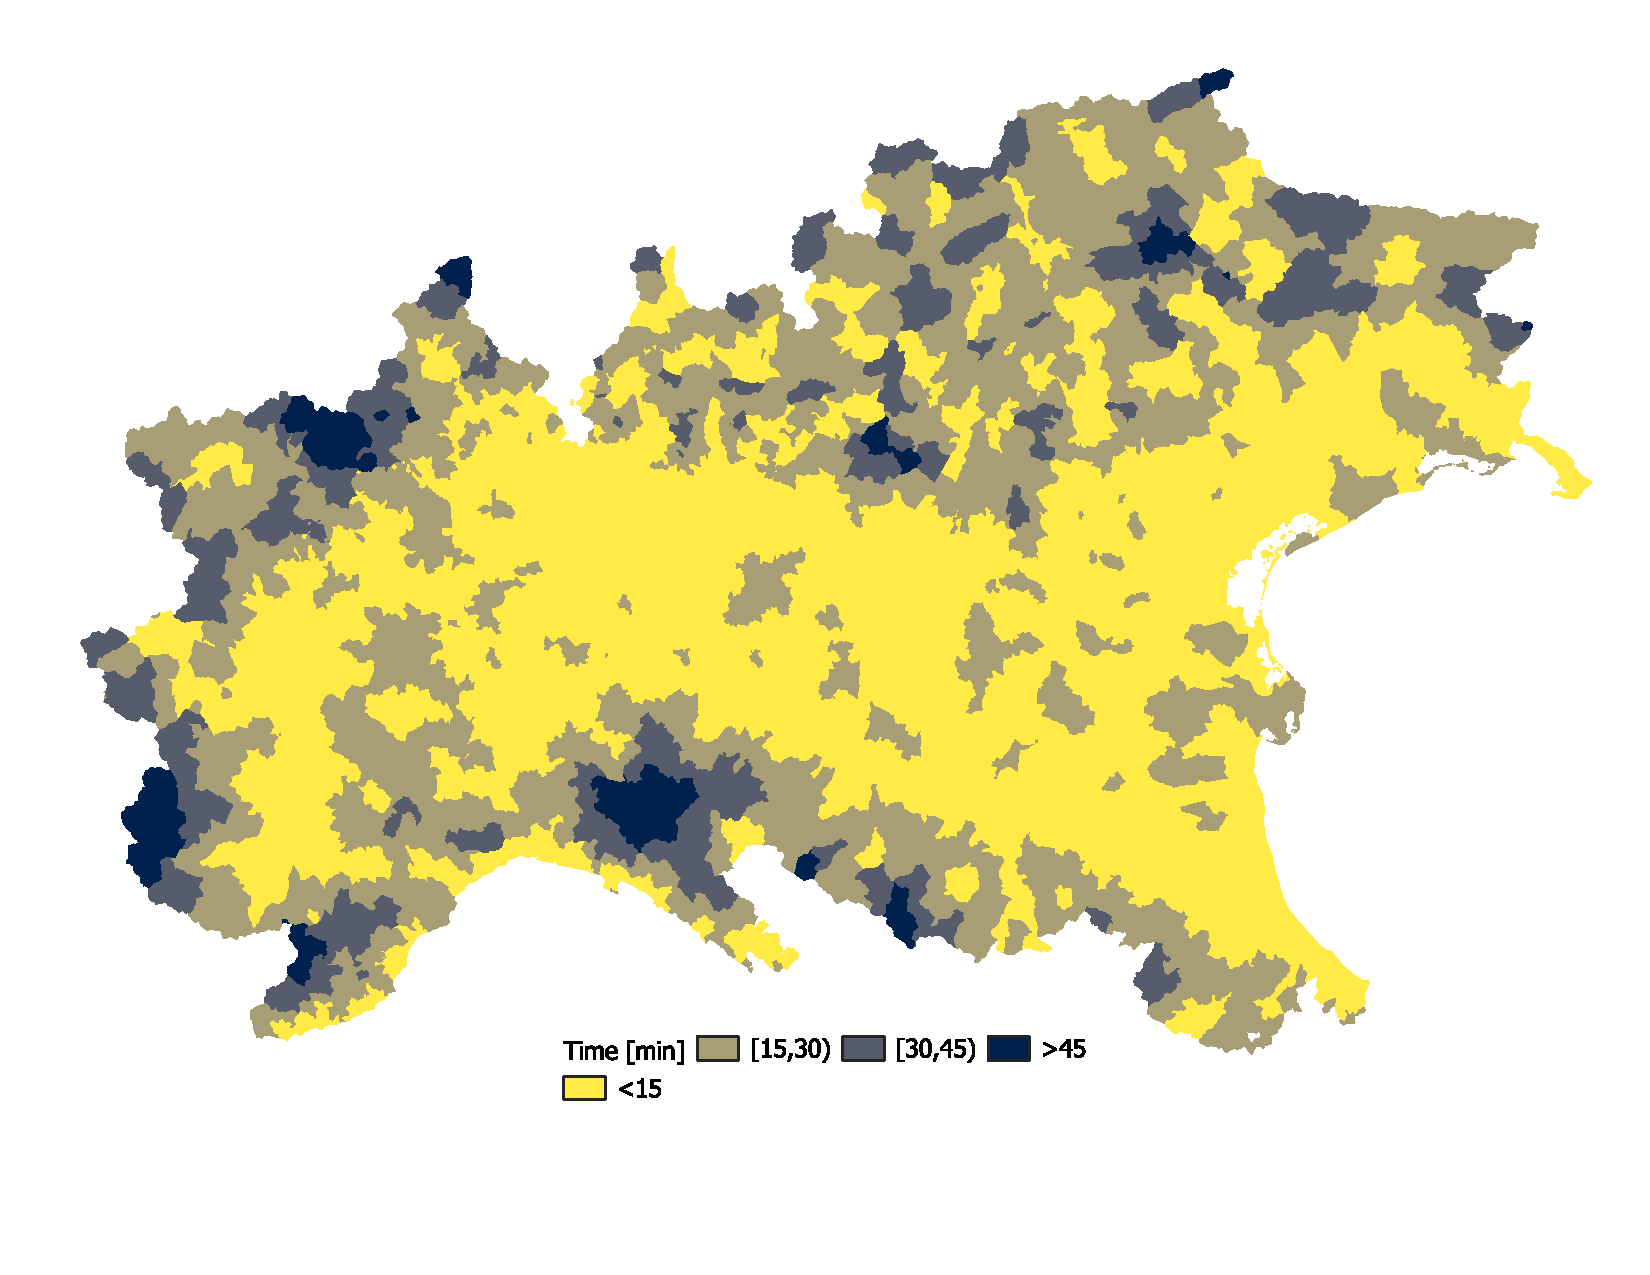
\includegraphics[height=0.8\textheight]{../report/img/Accessibilità per comune in 4 classi N.pdf}
		\caption{Accessibility to the closest healthcare service}
	\end{figure}
	
\end{frame}


\begin{frame}
	\frametitle{Accessibility in the North of Italy (2)}
	
	\begin{figure}[h]
		\centering
		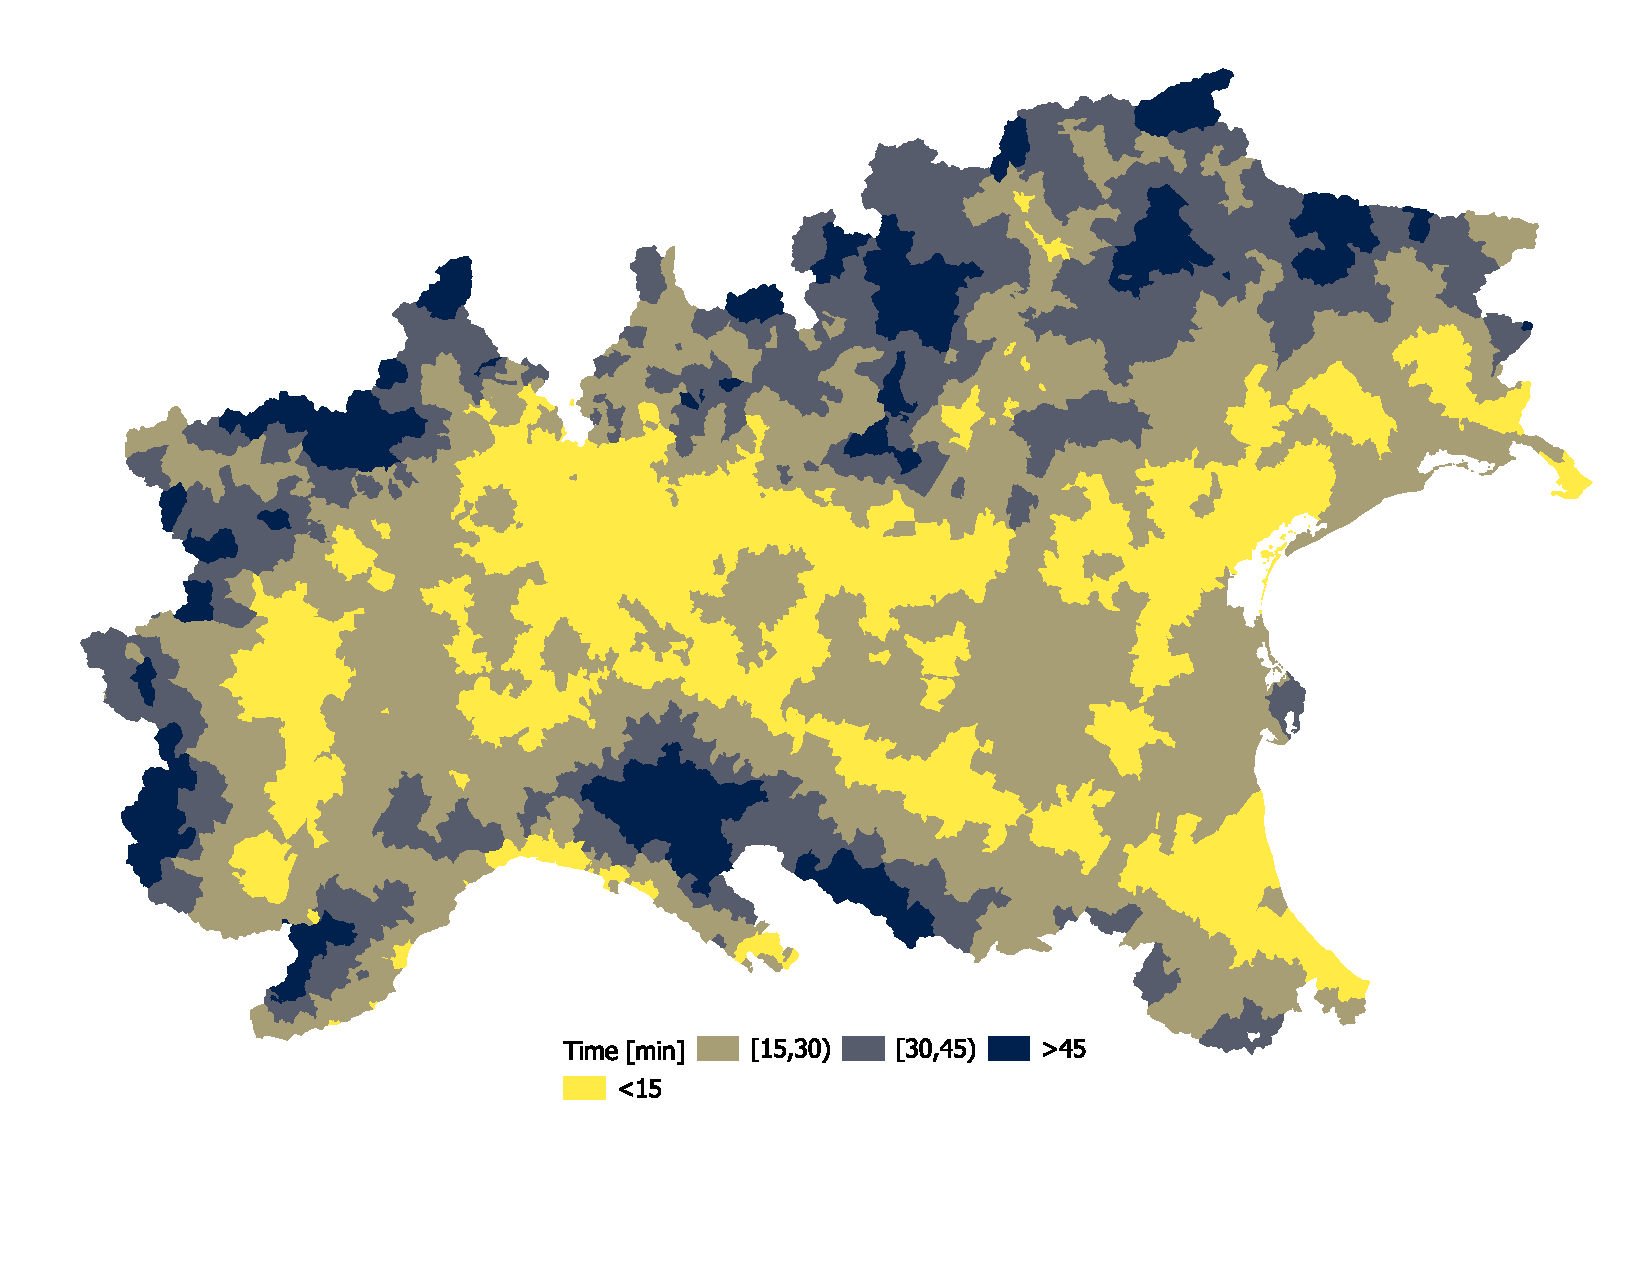
\includegraphics[height=0.8\textheight]{../report/img/Accessibilità per comune in 4 classi N 2023n3.pdf}
		\caption{Accessibility to the 3 closest healthcare services}
	\end{figure}
	
\end{frame}


\begin{frame}
	\frametitle{Distribution of municipalities by class}
	
	\begin{figure}[h]
		\centering
		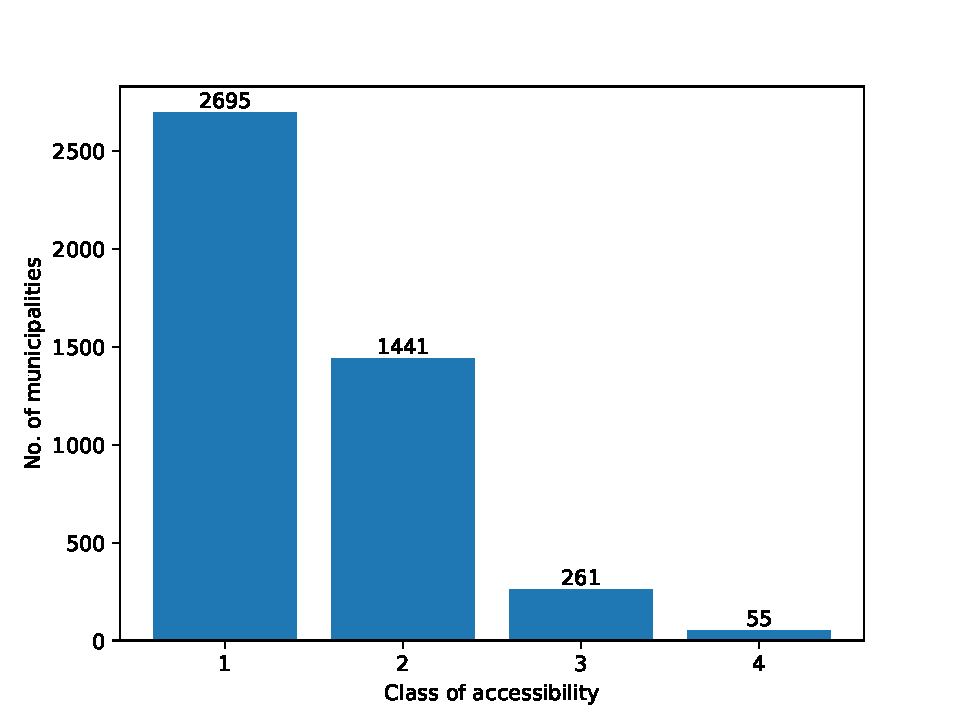
\includegraphics[height=0.7\textheight]{../report/img/acc_comm_by_class_North_2023n1.pdf}
		\caption{Time to reach the closest healthcare centre}
	\end{figure}
	
\end{frame}


\subsection{Population living in areas with low accessibility}

\begin{frame}
	\frametitle{Population in low accessibility areas}
	
	Share of population by accessibility area:
	\begin{center}
		\begin{tabular}{c c S[table-format=8.0] S[table-alignment-mode=marker]}
			\toprule
			\textbf{Class} & \textbf{Travel time} & \textbf{Population} & \textbf{\% of total}\\
			\midrule
			1 & < 15 & 18836153 & 69.32\\
			2 & [15, 30) & 7399725 & 27.23\\
			3 & [30, 45) & 792058 & 2.91\\
			4 & > 45 & 143979 & 0.53\\
			& &  27171915 & \\
			\bottomrule
		\end{tabular}
	\end{center}
	
\end{frame}


\begin{frame}
	\frametitle{Change in healthcare accessibility}
	
	7 intervals of change have been defined:
	\begin{center}
	\begin{tabular}{l c S[table-format=4.0] S[table-alignment-mode=marker]}
		\toprule
		\textbf{Class} & \textbf{Interval} & \textbf{Communes} & \\
		& \% & \text{No.} & \text{\%}\\
		\midrule
		Sharp improvement & $\leq -20$ & 135 & 3.03\\
		Relevant improvement & $\linterval{-20}{-10}$ & 348 & 7.82\\
		Slight improvement & $\linterval{-10}{-5}$ & 586 & 13.16\\
		No change & $\interval[open]{-5}{5}$ & 2298 & 51.62\\
		Slight worsening & $\rinterval{5}{10}$ & 494 & 11.1\\
		Relevant worsening & $\rinterval{10}{20}$ & 355 & 7.97\\
		Sharp worsening & $\geq 20$ & 236 & 5.3\\
		\bottomrule
		& & 4452 & \\
	\end{tabular}
	\end{center}
	
\end{frame}


\begin{frame}
	\frametitle{Variation between 2020 and 2023}
	
	Computed with this formula:
	\begin{equation*}
		\Delta_{n1} [\%] = \frac{\overline{t}_{2023n1} - \overline{t}_{2020n1}}{\overline{t}_{2020n1}} * 100
	\end{equation*}
	
	where\\[2ex]
	\begin{tabular}{c l}
		$\Delta$ & Variation as percentage\\
		$\overline{t}$ & Mean access time in the specified year\\
	\end{tabular}
	\bigskip
	
	Thus:
	\begin{align*}
		\Delta > 0 \quad & \Rightarrow \quad \text{worsening}\\
		\Delta < 0 \quad & \Rightarrow \quad \text{improvement} 
	\end{align*}
	
\end{frame}


\begin{frame}[containsverbatim]
	\frametitle{Formula implementation in SQL}
	
	The query executed to compute accessibility variation between 2020 and 2023:
	\medskip
	
	\begin{minted}{sql}
SELECT 
	c."COMM_ID",
	c."COMM_NAME",
	c.mean_health_2020_n1,
	c.mean_health_2023_n1,
	ROUND(((c.mean_health_2023_n1 - c.mean_health_2020_n1) / c.mean_health_2020_n1 * 100.0)::NUMERIC, 2) AS variation_n1,
	c.geom
FROM it_communes c
WHERE SUBSTRING(c."NUTS_CODE" FROM 1 FOR 3) IN ('ITC','ITH');
	\end{minted}
\end{frame}


\begin{frame}
	\frametitle{Map of changes}
	
	\begin{figure}[h]
		\centering
		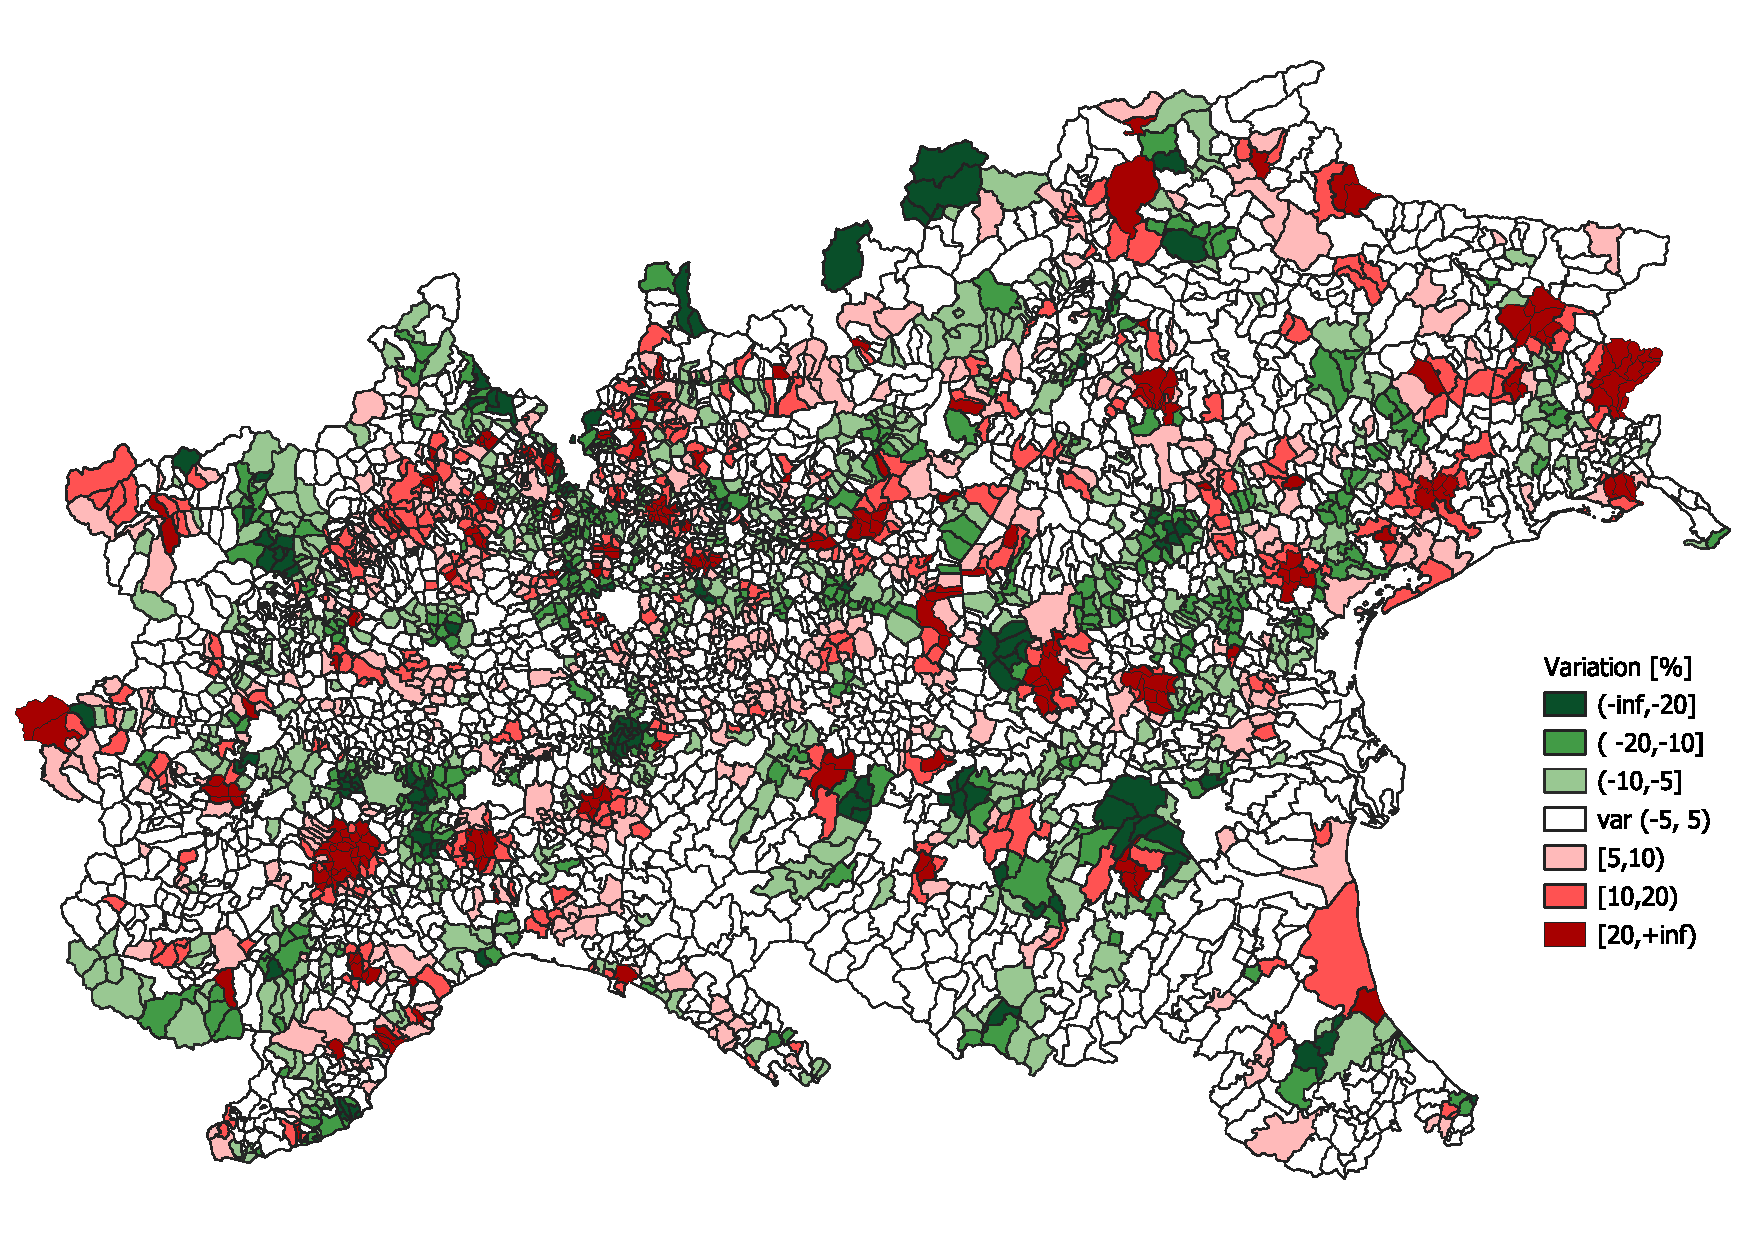
\includegraphics[height=0.8\textheight]{../report/img/var accessibilità n1 nord.pdf}
	\end{figure}
\end{frame}




